% The trident clause gadget for C = (x0 v x1 v x2), as in Fig. 2(c) of the
% paper. Build: pdflatex trident.tex ; pdftoppm -png -r 200 -singlefile trident.pdf trident
\documentclass[border=8pt]{standalone}
\usepackage{tikz}
\newcommand{\GT}{G_{\mathrm{T}}}
\newcommand{\GF}{G_{\mathrm{F}}}
\newcommand{\GB}{G_{\mathrm{B}}}
\begin{document}
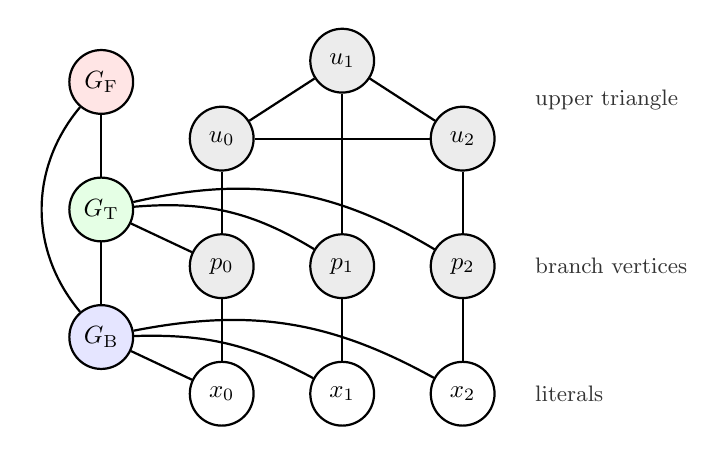
\begin{tikzpicture}[scale=0.9, transform shape,
    lit/.style={circle, draw, thick, minimum size=0.9cm, inner sep=0pt, font=\normalsize},
    loc/.style={circle, draw, thick, fill=gray!15, minimum size=0.9cm, inner sep=0pt, font=\normalsize},
    globt/.style={circle, draw, thick, fill=green!10, minimum size=0.9cm, inner sep=0pt, font=\bfseries\normalsize},
    globb/.style={circle, draw, thick, fill=blue!10, minimum size=0.9cm, inner sep=0pt, font=\bfseries\normalsize},
    globf/.style={circle, draw, thick, fill=red!10, minimum size=0.9cm, inner sep=0pt, font=\bfseries\normalsize},
    edge/.style={thick},
    note/.style={font=\small, gray!40!black, align=left}
]
    \node[globb] (GB) at (-1.7,0.8) {$\GB$};
    \node[globt] (GT) at (-1.7,2.6) {$\GT$};
    \node[globf] (GF) at (-1.7,4.4) {$\GF$};
    \draw[edge] (GB) -- (GT); \draw[edge] (GT) -- (GF); \draw[edge] (GF) to[bend right=40] (GB);
    \node[lit] (l0) at (0,0) {$x_0$}; \node[lit] (l1) at (1.7,0) {$x_1$}; \node[lit] (l2) at (3.4,0) {$x_2$};
    \draw[edge] (GB) -- (l0); \draw[edge] (GB) to[bend left=15] (l1); \draw[edge] (GB) to[bend left=20] (l2);
    \node[loc] (p0) at (0,1.8) {$p_0$}; \node[loc] (p1) at (1.7,1.8) {$p_1$}; \node[loc] (p2) at (3.4,1.8) {$p_2$};
    \node[loc] (u0) at (0,3.6) {$u_0$}; \node[loc] (u1) at (1.7,4.7) {$u_1$}; \node[loc] (u2) at (3.4,3.6) {$u_2$};
    \draw[edge] (l0) -- (p0); \draw[edge] (l1) -- (p1); \draw[edge] (l2) -- (p2);
    \draw[edge] (p0) -- (u0); \draw[edge] (p1) -- (u1); \draw[edge] (p2) -- (u2);
    \draw[edge] (u0) -- (u1); \draw[edge] (u1) -- (u2); \draw[edge] (u0) -- (u2);
    \draw[edge] (GT) -- (p0); \draw[edge] (GT) to[bend left=18] (p1); \draw[edge] (GT) to[bend left=22] (p2);
    \node[note, anchor=west] at (4.3,4.15) {upper triangle};
    \node[note, anchor=west] at (4.3,1.8) {branch vertices};
    \node[note, anchor=west] at (4.3,0) {literals};
\end{tikzpicture}
\end{document}
